%! TeX root = ../main.tex

\section{模型构建与实现}

\subsection{三个领域的职业选择}
对于职业的选择，我们并没有直接将此视为一种假设，而是将其视为一个优化问题。
将三个职业之间的差异性作为目标函数，目的是确保模型具有尽可能大的解释效度。
将“完备的数据支撑”与“政策相关性“作为约束条件，最终确保后续的模型均建立在基于数据的可复现的框架之上。

\subsubsection{基于O*NET的职业特征参数}
首先，我们需要将三个职业划定在三种特征维度上，依次为基础拉开三者的机制对比度，正好题目本身确定的三个领域具备这样的条件，于是我们参考得出三个职业的特征参数为 $\textit{digit}(x)$、$\textit{physical}(x)$ 和 $\textit{iprisk}(x)$ ，然后我们需要针对美国所有的职业在这三个维度上进行打分，为了避免主观赋值，我们采用美国劳工部维护的\textbf{O*NET}职业数据库\cite{onet2025database}作为统一数据源。
O*NET基于专家调查和从业者反馈，为每个职业提供大量\emph{数值量表descriptor}，大多数指标自然地给出在$0$--$100$之间的实数上，适合直接用于定量建模。

我们不试图为每个维度找到"唯一正确"的指标，针对每个特征轴，我们选择语义上能将O*NET描述符与三个维度直接对应起来的，且可下载的O*NET描述符\cite{onet2025database}，并将其用作该轴的代理变量，我们对于没有描述（descriptor字段缺失）的职业直接剔除。
基于以上约束，我们识别出三个主导维度
\begin{itemize}
    \item \textbf{数字化程度$digit(x)$}：核心任务可以以数字方式表示、自动化或增强的程度；
    \item \textbf{物理锚定$physical(x)$}：任务执行对现场物理存在或与环境的手动交互的依赖程度；
    \item \textbf{知识产权和署名风险$iprisk(x)$}：价值创造对作者身份、原创性和所有权的敏感程度。
\end{itemize}

表~\ref{tab:onet_descriptor_mapping} 列出了每个特征轴所对应的O*NET描述符及说明。

\begin{table}[H]
\centering
\caption{三维特征轴与O*NET描述符的对应关系}
\label{tab:onet_descriptor_mapping}
\begin{tabular}{@{}>{\raggedright\arraybackslash}p{2.2cm} >{\raggedright\arraybackslash}p{4.0cm} >{\raggedright\arraybackslash}p{4.8cm} >{\raggedright\arraybackslash}p{3.0cm}@{}}
\toprule
\textbf{特征轴} & \textbf{客观取值方式} & \textbf{O*NET描述符} & \textbf{合理性说明} \\
\midrule
$digit(x)$\newline 数字化程度 & 工作行为中对计算机/电子媒介的依赖 & Working with Computers~\cite{onetWorkingWithComputers}；\newline E-Mail~\cite{onetEmail} & 直接刻画工作是否以计算机与电子信息流为主 \\
\addlinespace
$physical(x)$\newline 物理锚定程度 & 手部操作+身体姿态负担等物理现场需求 & Using Hands to Handle Objects~\cite{onetUsingHands}；\newline Kneeling/Crouching~\cite{onetKneeling} & 直接量化现场动手强度与工位姿态限制 \\
\addlinespace
$iprisk(x)$\newline 产权/归因风险 & 产出是否以原创表达/创意贡献为核心 & Originality~\cite{onetOriginality}；\newline Thinking Creatively~\cite{onetThinkingCreatively} & 用原创表达强度作为可复现的风险代理变量 \\
\bottomrule
\end{tabular}
\end{table}

基于此，筛选出同时具备以上6个描述符字段的所有职业，对于每个职业 $x$，O*NET均提供了对应的描述符的评分，于是令 $v_m(x)$ 表示其在O*NET描述符 $m$ 下的原始评分（$0$--$100$）。
我们在整个职业集上应用最小-最大归一化：
\begin{equation}
    z_m(x)=\frac{v_m(x)-\min_{y}v_m(y)}{\max_{y}v_m(y)-\min_{y}v_m(y)} \in [0,1],
\end{equation}
其中 $y$ 遍历所有职业。设特征轴 $k \in \{digit, physical, iprisk\}$ 对应的描述符集合为 $D_k$（见表~\ref{tab:onet_descriptor_mapping}），则对同一特征轴下的多个描述符取等权平均：
\begin{equation}
    \textit{feature}_k(x) = \frac{1}{|D_k|} \sum_{m \in D_k} z_m(x).
\end{equation}
由此得到 $\textit{digit}(x)$、$\textit{physical}(x)$ 和 $\textit{iprisk}(x)$的数值。

每个候选职业$x$由一个归一化的三维特征向量表示，作为作为3Dscatter中的一个数据点。
\begin{equation}
    f(x)=\big(digit(x),\,physical(x),\,iprisk(x)\big)\in[0,1]^3,
\end{equation}
为了选出符合条件的职业中，三个能够构成最大异质性（差异性）的职业，考虑从几何角度出发，找到三个在三维坐标系中构成最大三角平面的数据点，于是按照标准面积计算公式有：

\begin{equation}
Area3D(x_S, x_T, x_A) = \frac{1}{2} \left\lVert \big(f(x_T) - f(x_S)\big) \times \big(f(x_A) - f(x_S)\big) \right\rVert_{2}
\label{eq:area3d}
\end{equation}
其中 $x_S \in \text{STEM}$ ，$x_T \in \text{Trade}$ ，$x_A \in \text{Arts}$ 。\\

%（公式已移至附录，详见附录~\ref{appendix:area2d_formula}。此处不再赘述。）
然后通过Python进行可视化（图~\ref{fig:heterogeneity3d} 和图~\ref{fig:heterogeneity2d}）。

\vspace*{-3em} % 根据版式适当调整消耗空白空间的高度。可微调 -3em 为合适数值。
\begin{figure}[H]
\centering
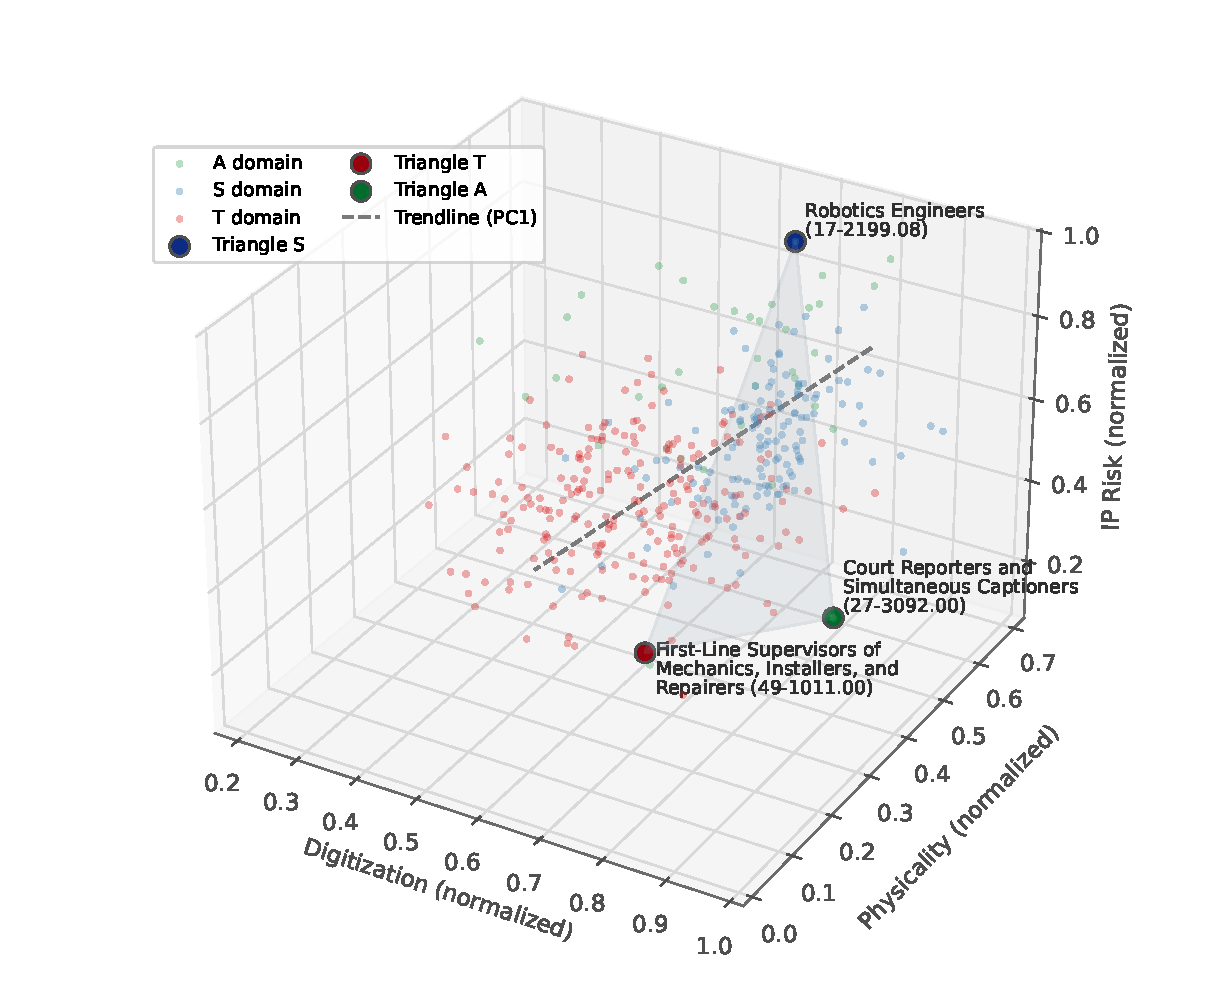
\includegraphics[width=0.93\textwidth]{figures/fig_heterogeneity_3d_all_points_strict_tight.pdf}
\caption{全体职业三维异质性点云与最优三角面（基于归一化后的O*NET描述符）}
\label{fig:heterogeneity3d}
\end{figure}

我们先在全点云上求解无约束的最大面积三角形，但结果中包含的某一职业并未被官方纳入三个领域中的任何一个。因此，我们在可行域内加入必须属于 O*NET 维护的目标领域的约束，最终得到约束下的最优三点分别为 STEM（Robotics Engineers）、技工/Trades（First-Line Supervisors of Mechanics, Installers, and Repairers）与艺术/媒体（Court Reporters and Simultaneous Captioners）。三者构成的三角形面积为 $0.262221$。

如图~\ref{fig:heterogeneity3d} 所示，三维散点图直观展示了最终优化结果。为了体现职业之间的两两异质性，我们进一步绘制了该点云的二维投影，见图~\ref{fig:heterogeneity2d}。

\vspace{0.6\baselineskip}

\begin{figure}[H]
\centering
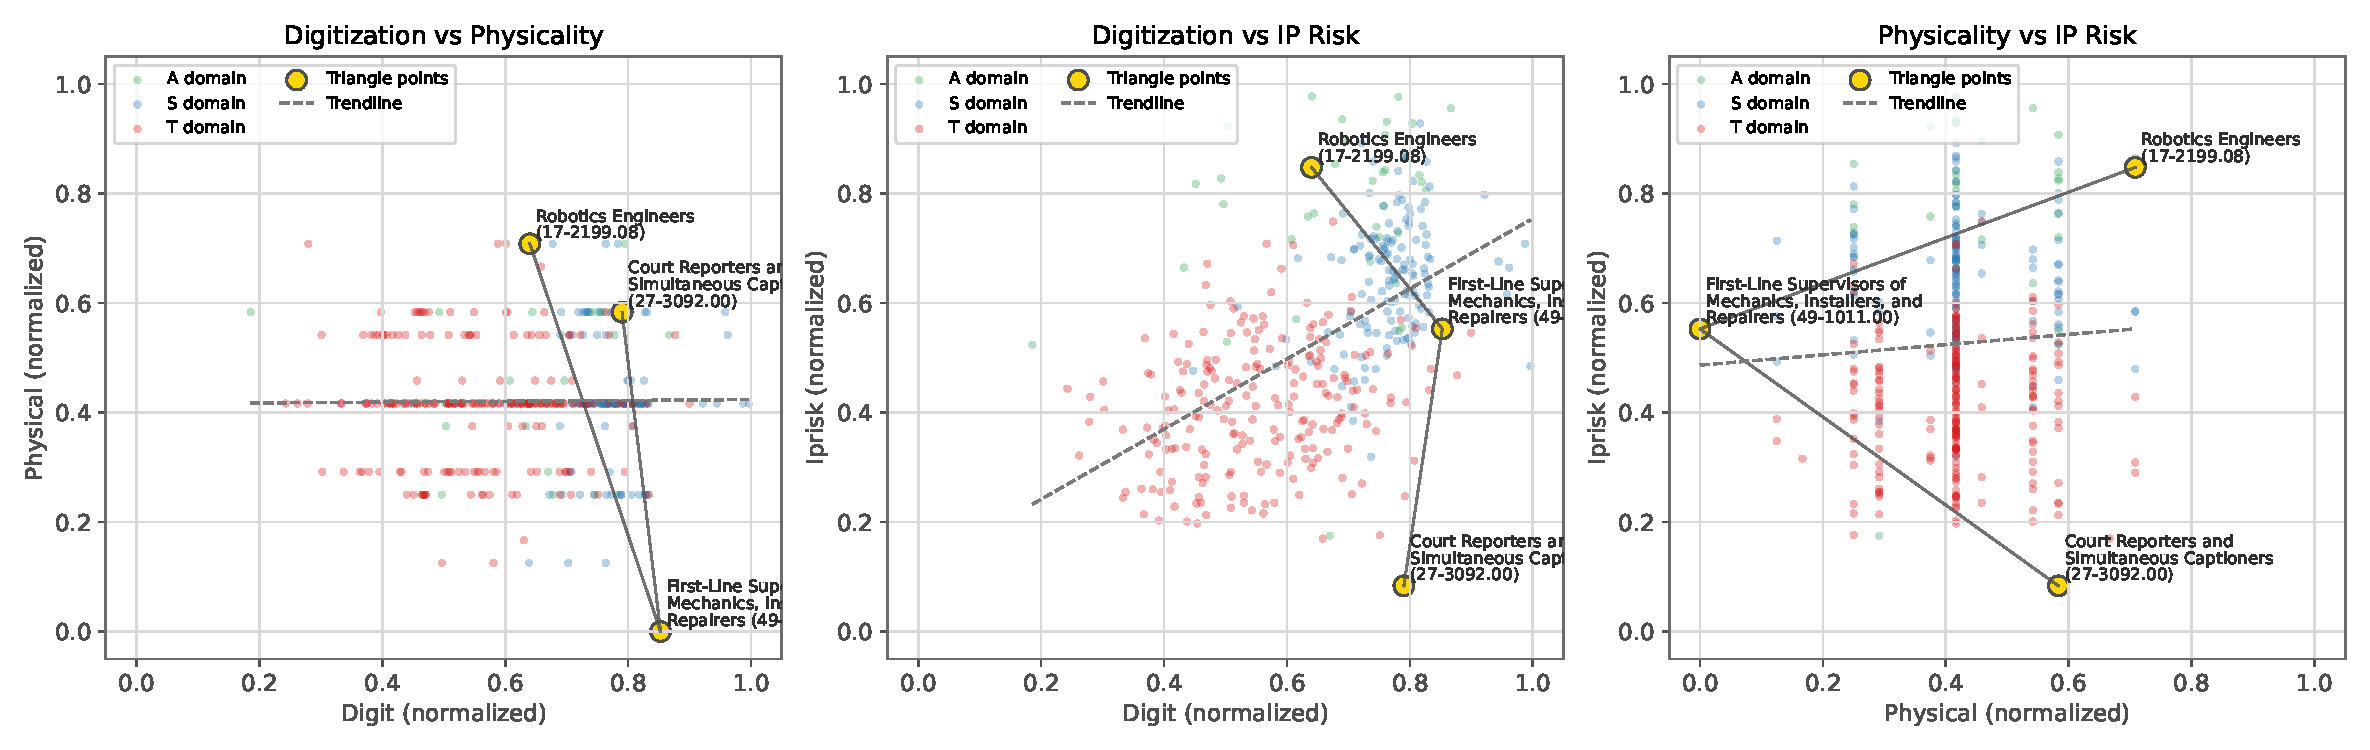
\includegraphics[width=0.92\textwidth]{figures/fig_heterogeneity_2d_projections_all_points_strict.pdf}
\caption{全体职业异质性空间的二维投影与最优三点标注（二维面积公式见附录~\ref{appendix:area2d_formula}）}
\label{fig:heterogeneity2d}
\end{figure}

针对二维投影进行分析：Robotics Engineers的数字化略低于Court Reporters and Simultaneous Captioners，并且位于高物理性、高知识产权风险区域；First-Line Supervisors of Mechanics, Installers, and Repairers位于低物理性、中等知识产权风险区域；而Court Reporters and Simultaneous Captioners则位于中等物理性、低知识产权风险区域。可见三种职业在任意两维组合下均保持较大的差异性，将其作为三个领域代表具有合理性。（三者的O*NET-SOC 代码分别为：STEM：17-2199.08；Trade：49-1011.00；Arts：27-3092.00）。

\subsection{职业演化的模型构建}

问题的第二个核心要求是为所选的三个职业构建一个\emph{数据驱动}的未来演化模型，并强调了结合“当前轨迹（current trajectory）”以及相关的驱动因素。
首先，从第一性原理出发，职业是由其任务组成（DNA）所定义的，因此在Gen-AI的影响下，其未来的Task DNA必定会发生结构上的“变异”，因此，试图预测未来的该职业的岗位需求本身逻辑上就存在问题，因为彼时的职业已经非此时的职业了。\\
所以，我们并不会直接预测未来职业的岗位需求，而是从更本质的角度出发，研究在当前Gen-AI发展轨迹下，未来职业的Task DNA的结构变化。为了便于理解，我们绘制图~\ref{fig:task_redefinition} 来展示职业的演化流程。

\begin{figure}[htbp]
\centering
\begin{tikzpicture}[
  node distance=2.4cm,
  box/.style={draw=gray!70, rounded corners=2pt, minimum width=3.2cm, minimum height=1.0cm, align=center},
  mid/.style={draw=gray!70, rounded corners=2pt, minimum width=3.2cm, minimum height=1.0cm, align=center, fill=gray!5},
  arrow/.style={-Latex, line width=0.8pt, color=gray!80}
]
  \node[box] (jobA) {职业A\\(原有结构)};
  \node[mid, right=of jobA] (mutation) {结构变异};
  \node[box, right=of mutation] (jobB) {职业B\\(重定义后)};

  \draw[arrow] (jobA) -- node[above, align=center, font=\small, text=gray!80] {Gen-AI影响} (mutation);
  \draw[arrow] (mutation) -- node[above, align=center, font=\small, text=gray!80] {职业重定义} (jobB);

  \coordinate (progressLeft) at ($(jobA.south west)+(0,-0.6)$);
  \coordinate (progressRight) at ($(jobB.south east)+(0,-0.6)$);
  \coordinate (progressMid) at ($(progressLeft)!0.5!(progressRight)$);
  \draw[arrow] (progressLeft) -- ($(progressMid)+(-0.6,0)$);
  \draw[arrow] ($(progressMid)+(0.6,0)$) -- (progressRight);
  \node[font=\small, text=gray!80] at (progressMid) {发展趋势};
\end{tikzpicture}
\caption{任务结构重排导致职业重定义的演绎路径}
\label{fig:task_redefinition}
\end{figure}



由于官方给出的职业的原始任务描述字段太多，因此构建 Task DNA 的任务权重 $w_{ij}$，结合权威数据来源，在任务（而非职业）层面，计算其替代/增强强度 $(s_{ij},c_{ij})$，进而得到该职业的任务级净冲击为
\begin{equation}
    \mu_{ij}^{task}=c_{ij}-s_{ij},
\end{equation}
并将“当前轨迹”定义为外生采纳路径 $A(t)\in[0,1]$（快速/中速/慢速三种情景），用于驱动任务需求随时间的演化。

\vspace{0.5\baselineskip}

% \subsubsection{未来演化的可计算定义}
% 我们基于“没有人能准确预测未来某个具体时间节点的定量变化”原则，转而采用更广义的时间跨度来预测定性的变化。\\
% 对此，我们定义当某个关键任务在职业内的相对需求（份额）下降至一个足够小的阈值 $\epsilon$ 以下时，即认为该任务在可操作意义上“趋近于消失”。
% 具体地，若 $p_{ij}(t)$ 表示职业 $i$ 中任务 $j$ 在时刻 $t$ 的相对需求份额（定义见后文），则定义任务 $j$ 的“有效归零时间”为
% \begin{equation}
%     \tau_{ij}(\epsilon)=\min\{t:\ p_{ij}(t)\le \epsilon\}.
% \end{equation}
% 该定义可直接用于回答“未来何时发生显著变化”的问题，并允许通过不同 $\epsilon$ 取值进行敏感性分析。

\subsubsection{任务层动态预测模型}

在上述论证之后，我们给出任务层预测的数学公式。
模型包含两类输入：\textbf{任务结构}（来自O*NET任务数据）与\textbf{发展轨迹}（GenAI采纳路径 $A(t)$）。
预测输出为：每个职业内部任务的相对需求演化 $p_{ij}(t)$，以及“有效归零时间” $\tau_{ij}(\epsilon)$。

\paragraph{任务结构（Task DNA）与任务净冲击}

\paragraph{任务DNA的定义与数据来源}
对于职业 $i$，我们需要选取其\textbf{前N项核心任务}作为其任务DNA（任务索引 $j = 1, \ldots, 20$）。每项任务 $j$ 取自O*NET对于此职业的任务描述 $Task_j$\cite{onet2025database}，该数据库对于每个职业的任务构成都有相应的重要性和频率评分数据，因此我们定义两个基于该数据的描述符：
\textbf{任务重要性} $IM_j$（范围 0--100）；
\textbf{任务频率} $FR_j$（范围 0--100，或同等的频率量表）。\\


我们将任务权重定义为重要性 $IM_j$ 与频率 $FR_j$ 乘积的归一化值。令未归一化的权重为：
\begin{equation}
    \tilde{w}_j = IM_j \cdot FR_j,
\end{equation}
然后通过下式进行归一化：
\begin{equation}
    w_{ij} = \frac{\tilde{w}_j}{\sum_{k=1}^{20} \tilde{w}_k}, \quad \sum_{j=1}^{20} w_j = 1.
\end{equation}

进一步的，通过Python编程（如果所选SOC（标准职业分类）代码缺少任务频率量表 $FR_j$，则仅使用重要性值（即设 $\tilde{w}_j = IM_j$））。得到三个职业的Top Task（20个以内），将其可视化，分布见图~\ref{fig:task_dna_imfr_triptych}，任务文本图例见附录~\ref{app:task_dna_figures}。

\begin{figure}[H]
\centering
\begin{minipage}{0.32\linewidth}
    \centering
    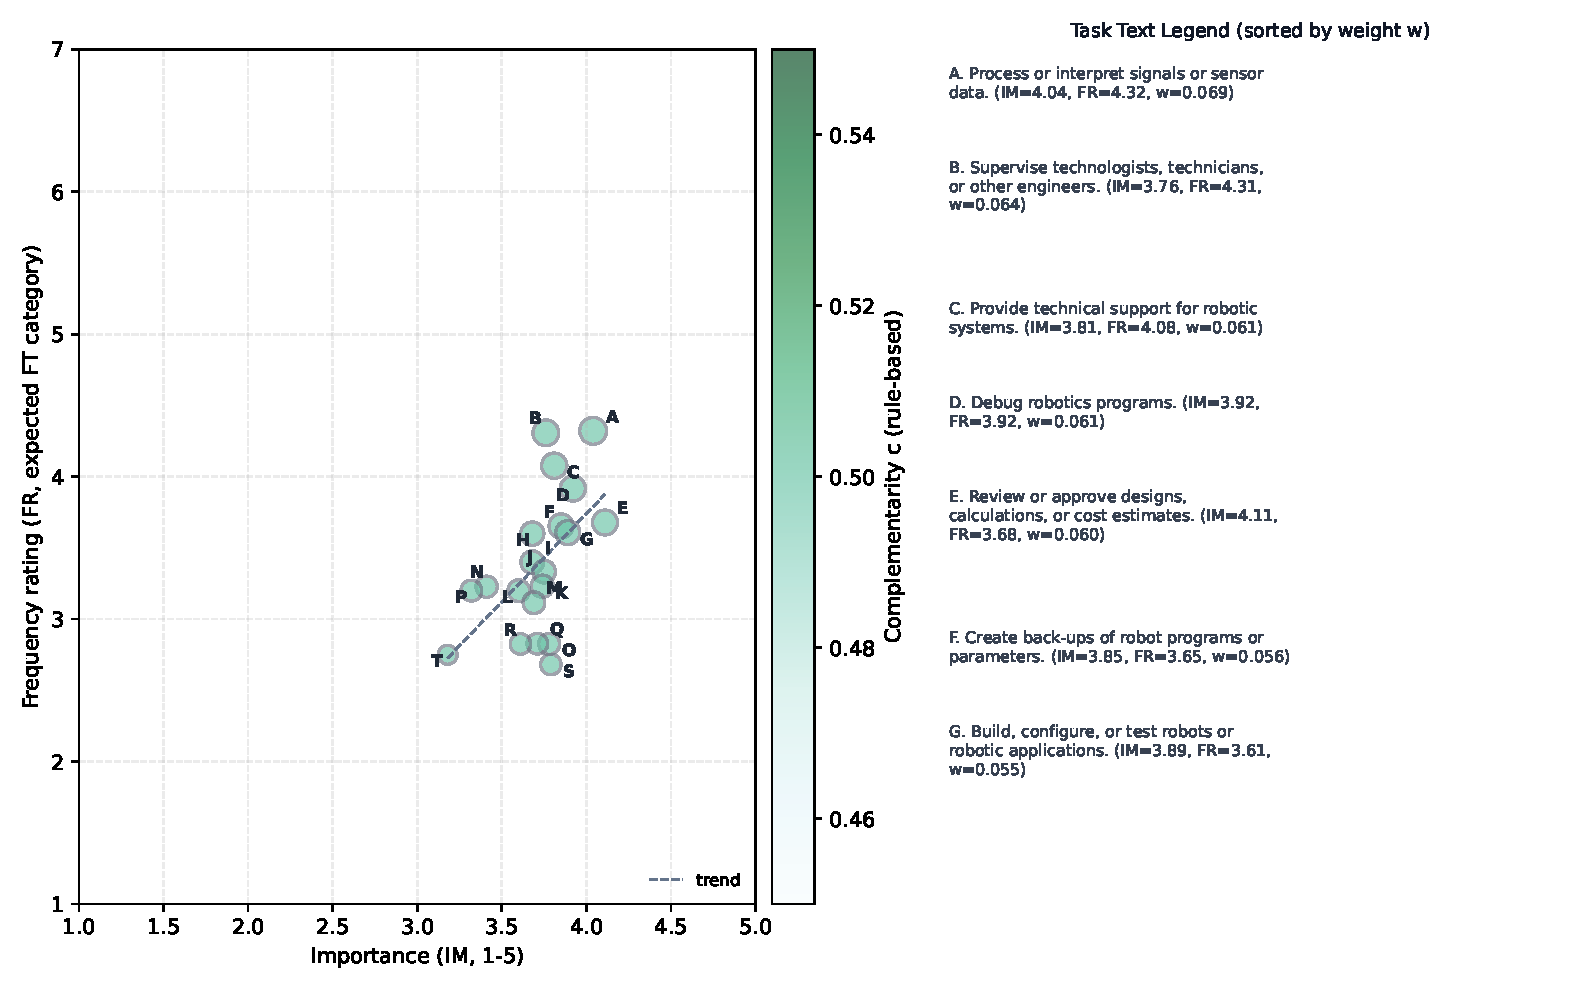
\includegraphics[width=\linewidth]{figures/task_dna_17-2199.08_weights.pdf}\\
    \small (a) 17-2199.08 机器人工程师
\end{minipage}\hfill
\begin{minipage}{0.32\linewidth}
    \centering
    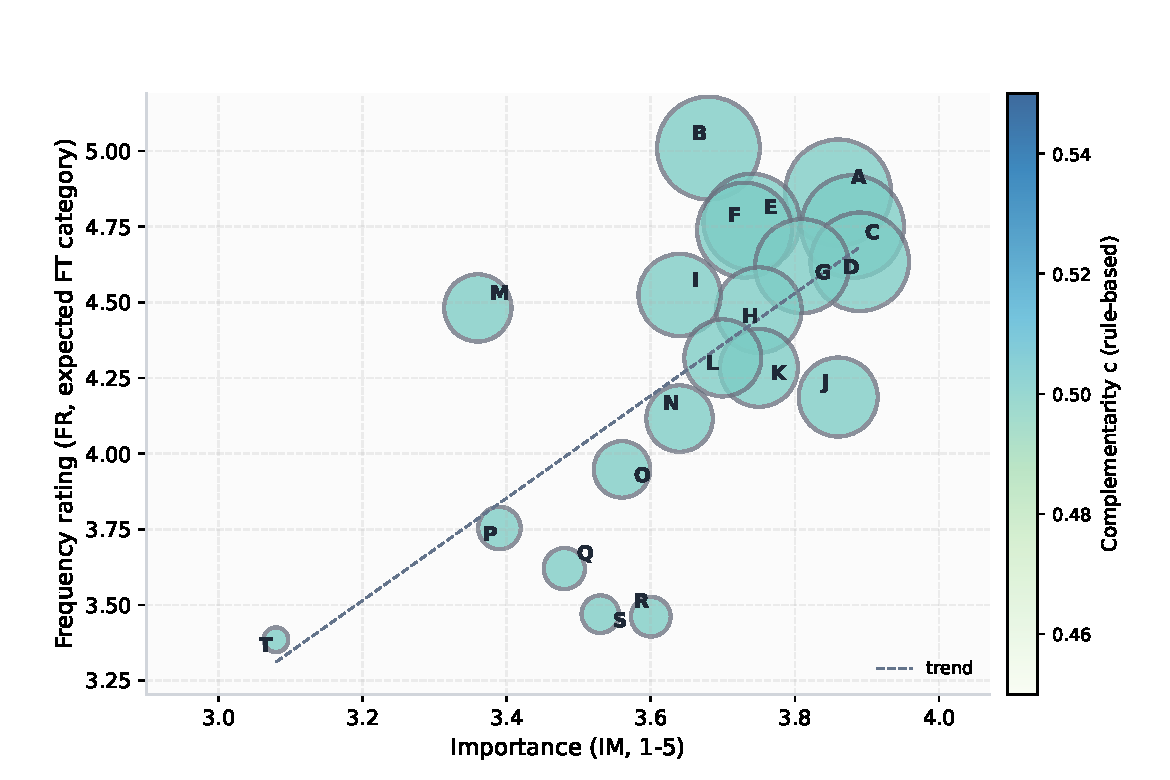
\includegraphics[width=\linewidth]{figures/task_dna_49-1011.00_weights.pdf}\\
    \small (b) 49-1011.00 一线主管
\end{minipage}\hfill
\begin{minipage}{0.32\linewidth}
    \centering
    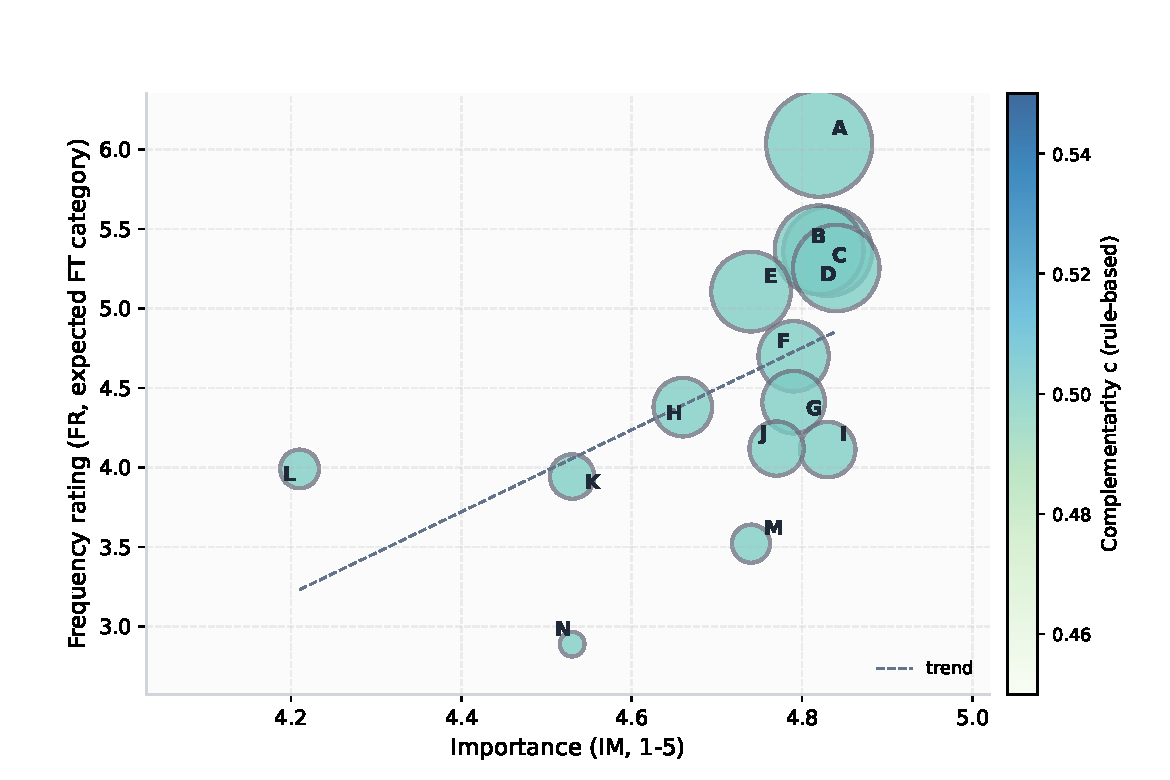
\includegraphics[width=\linewidth]{figures/task_dna_27-3092.00_weights.pdf}\\
    \small (c) 27-3092.00 法庭速录
\end{minipage}
\caption{三个职业任务DNA权重分布（IM--FR 散点图），点面积与 $w_j$ 成正比。字母对应的文本图例见附录~\ref{app:task_dna_figures}。}
\label{fig:task_dna_imfr_triptych}
\end{figure}


结合三类职业的Task DNA，进一步给出针对性的解释：对于\textbf{机器人工程师}，其职业价值主要由少数高权重技术任务驱动；对于\textbf{一线主管（机械/安装/维修）}，点更分散且中等权重任务占比更高，反映管理、协调、现场判断等任务的多元并存，模型上对应更平缓的权重梯度，结构变化由多项任务共同贡献；而\textbf{法庭速录与字幕}高度依赖少数语言处理核心任务。

得到三个职业的Top Task后，我们将其与当前Gen-AI能力进行映射，进而研究每一个Task受到的影响强度。\\
首先我们同样需要对当今Gen-AI的能力进行解剖，划分出多个能力维度。以下的三点为主要的划分依据：

\begin{itemize}
    \item 覆盖主要工作活动类型：从技术问题解决到语言处理，涵盖职业任务的主要类别
    \item 可量化可审计：每个维度都有对应的权威基准测试，避免主观评估
    \item 与当前三个职业的任务构成相匹配：每个Task DNA都能通过公开的 AI 测试分数来衡量。
\end{itemize}

为避免主观的连续评分，我们针对能力分段（$M_k$）构建一个横向的离散能力等级：
\begin{itemize}[label={},leftmargin=*]
    \item[] 高（$\ge 0.85$）\quad
    较高（$0.70$--$0.85$）\quad
    中等（$0.50$--$0.70$）\quad
    低（$0.30$--$0.50$）\quad
    极低（$<0.30$）
\end{itemize}
并在每个区间内取代表值 $M_k$（具体映射见表~\ref{tab:genai_scale}）。

同时引入{方向系数（$\rho_k$）}刻画“替代/互补/平衡”的偏向强度，若
$\rho_k<0$：则偏替代（AI可独立完成可交付物）；
若$\rho_k>0$：则偏互补（AI提供建议/辅助，人必须在环）；
若$\rho_k=0$：则平衡（两边都强，净效应不确定）。
\\
\ $M_k$ 选取当前顶尖模型在相关指标上的代表性得分（0$\sim$1标准化后）。$\rho_k = c_k - s_k$ 表示GenAI对该维度的影响方向：正值为互补（提升人效使需求上升），负值为替代（可自动化使需求下降）。

最终将结果汇总至表~\ref{tab:genai_scale}。
\begin{table}[H]
\centering
\caption[GenAI 九维能力映射总表]{GenAI 九维能力映射总表}
\label{tab:genai_scale}
\small
\setlength{\tabcolsep}{2pt}
\renewcommand{\arraystretch}{1.15}
\setlength{\extrarowheight}{2pt}
\resizebox{\textwidth}{!}{%
\begin{tabular}{p{2.6cm} p{3.6cm} p{4.6cm} | p{1.0cm} p{2.2cm} p{1.0cm} p{0.9cm} p{0.9cm}}
\toprule
\textbf{维度（编号）} & \textbf{定义} & \textbf{代表性指标（来源 \& 分数）} & \textbf{$M_k$} & \textbf{能力等级（阈值规则）} & \textbf{$\rho_k$} & \textbf{$s_k$} & \textbf{$c_k$} \\
\midrule
D1 工程技术问题解决 &
运用工程知识分析解决技术问题（调试维护、技术支持） &
MMLU 86.4\%；ARC 96.3\%（GPT-4 报告\citep{openai2023gpt4}） &
0.90 & 高（$\ge 0.85$） & $+0.35$ & 0.50 & 0.85 \\
D2 数据分析与评估 &
分析传感器/数值数据并据标准评估（质检、数据监控） &
GSM8K 92.0\%；DROP 80.9（GPT-4 报告\citep{openai2023gpt4}） &
0.80 & 较高（$0.70$--$0.85$） & $+0.20$ & 0.30 & 0.50 \\
D3 算法编程与自动化 &
编写和修正代码脚本实现需求（软件算法开发、自动化流程） &
HumanEval 67.0\%；SWE-bench 修复 20\%\citep{openaicodex2021,swebench2024} &
0.67 & 中等（$0.50$--$0.70$） & $-0.20$ & 0.90 & 0.70 \\
D4 现场感知与物理操作 &
感知物理环境及动手操作设备（现场检查、安全监督、设备调校） &
AutoGPT 实体环境任务 24\%；视觉识别 $\approx 85\%+$\citep{autogpt2023,imagenet2009} &
0.25 & 低（$0.30$--$0.50$） & $+0.40$ & 0.10 & 0.50 \\
D5 规划与流程调度 &
制定任务计划、优化流程顺序和资源分配（调度排程、进度管理） &
AutoGPT 自主任务完成率 $\sim 65\%$；工具使用成功率 $\sim 80\%$\citep{autogpt2023} &
0.65 & 中等（$0.50$--$0.70$） & $-0.10$ & 0.60 & 0.50 \\
D6 协作沟通与培训 &
沟通协作、传授知识并协调团队（培训、跨部门协作） &
人类偏好：GPT-4 胜率 70.2\%\citep{openai2023gpt4} &
0.70 & 较高（$0.70$--$0.85$） & $+0.45$ & 0.30 & 0.75 \\
D7 监督管理与质量控制 &
监督工作表现并确保质量达标（绩效管理、质检） &
HellaSwag 95.3\%\citep{openai2023gpt4} &
0.80 & 较高（$0.70$--$0.85$） & 0.00 & 0.68 & 0.68 \\
D8 语言理解与文本生成 &
理解口语/文本并生成书面内容（转录、写作、翻译） &
Whisper WER $\approx 0.011$；GPT-4 文本偏好胜率 70\%\citep{whisper2022,openai2023gpt4} &
0.95 & 高（$\ge 0.85$） & $-0.40$ & 0.90 & 0.50 \\
D9 信息管理与检索 &
有序存储组织信息并按需高速检索核验（档案管理、查询答复） &
DocVQA 99.16\%；Text-to-SQL $>80\%$\citep{docvqa2017,spider2018} &
0.90 & 高（$\ge 0.85$） & 0.00 & 0.30 & 0.30 \\
\bottomrule
\end{tabular}}

\end{table}
\begin{spacing}{0.9}
\noindent
\textbf{注：}D9 的 DocVQA 99.16\% 可视为文档问答场景的上界证据，不等价于所有检索情境与数据库规模下的通用能力。D4/D5 采用 AutoGPT 端到端完成率与工具使用成功率作为下界证据，用于避免夸大“现场操作/流程调度”的可自动化程度。

上表只展示了Gen-AI的九个维度，而
图~\ref{fig:genai_taskdna_chord_robotics}为映射关系的更直观展示。
\begin{figure}[H]
\centering
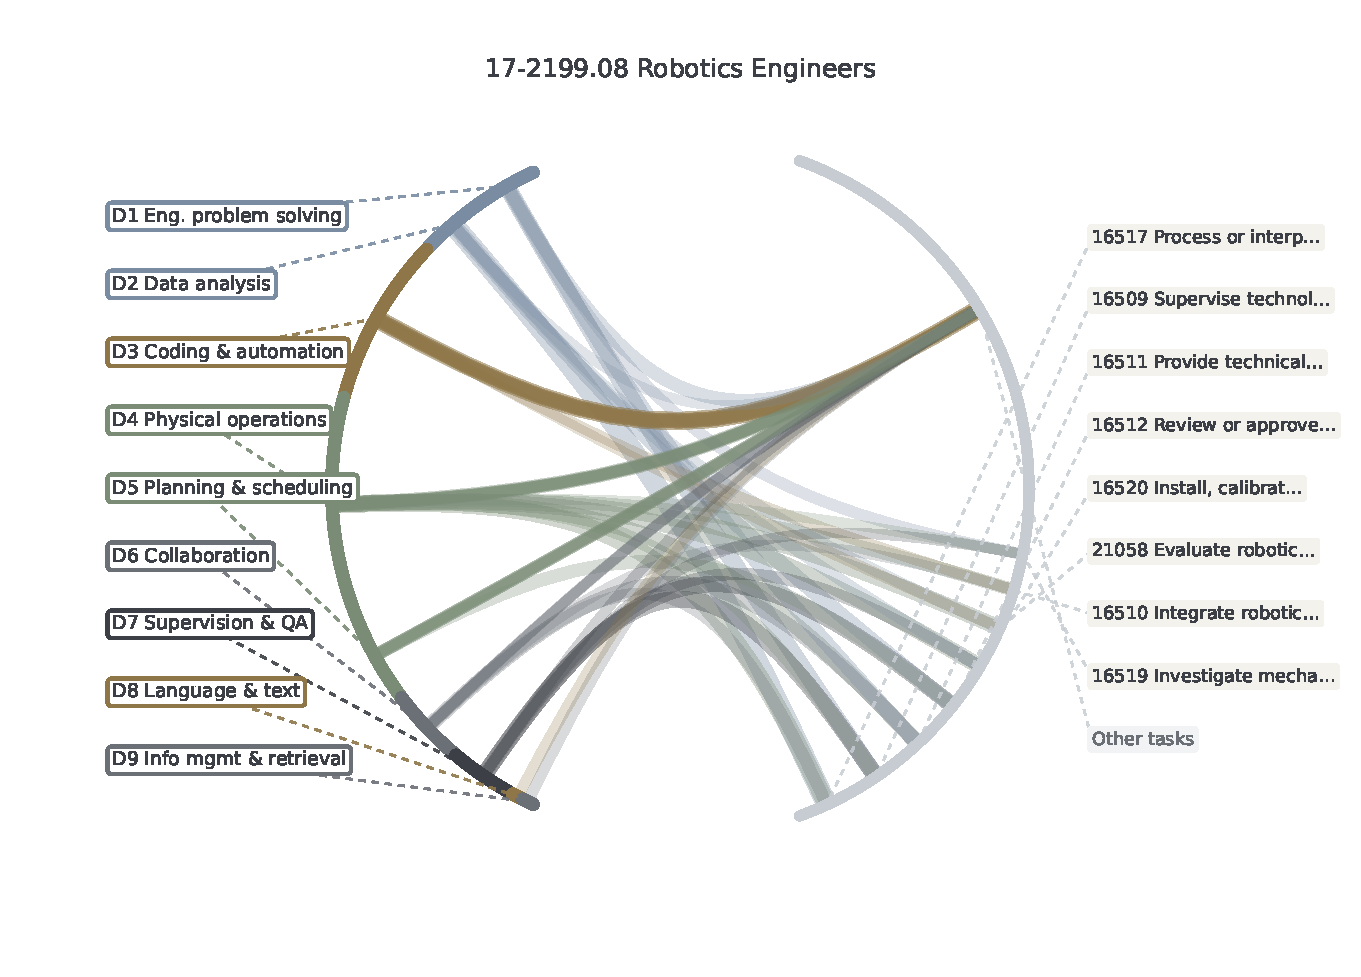
\includegraphics[width=0.86\textwidth]{figures/fig_genai_taskdna_chord_17-2199.08.pdf}
\caption{GenAI 能力 $\rightarrow$ Task DNA 映射弦图（机器人工程师，17-2199.08）。}
\label{fig:genai_taskdna_chord_robotics}
\end{figure}


总的来看，GenAI 在语言和编码等维度能力较高，呈现替代趋势，而在涉及物理、管理等维度时，仍主要作为辅助工具，与人类技能形成互补。
\end{spacing}

% 为了更直观的显示Gen-AI能力对三个职业的task的映射，我们绘制了图~\ref{fig:task_dna_genai_mapping_triptych}。


% \begin{figure}[H]
% \centering
% 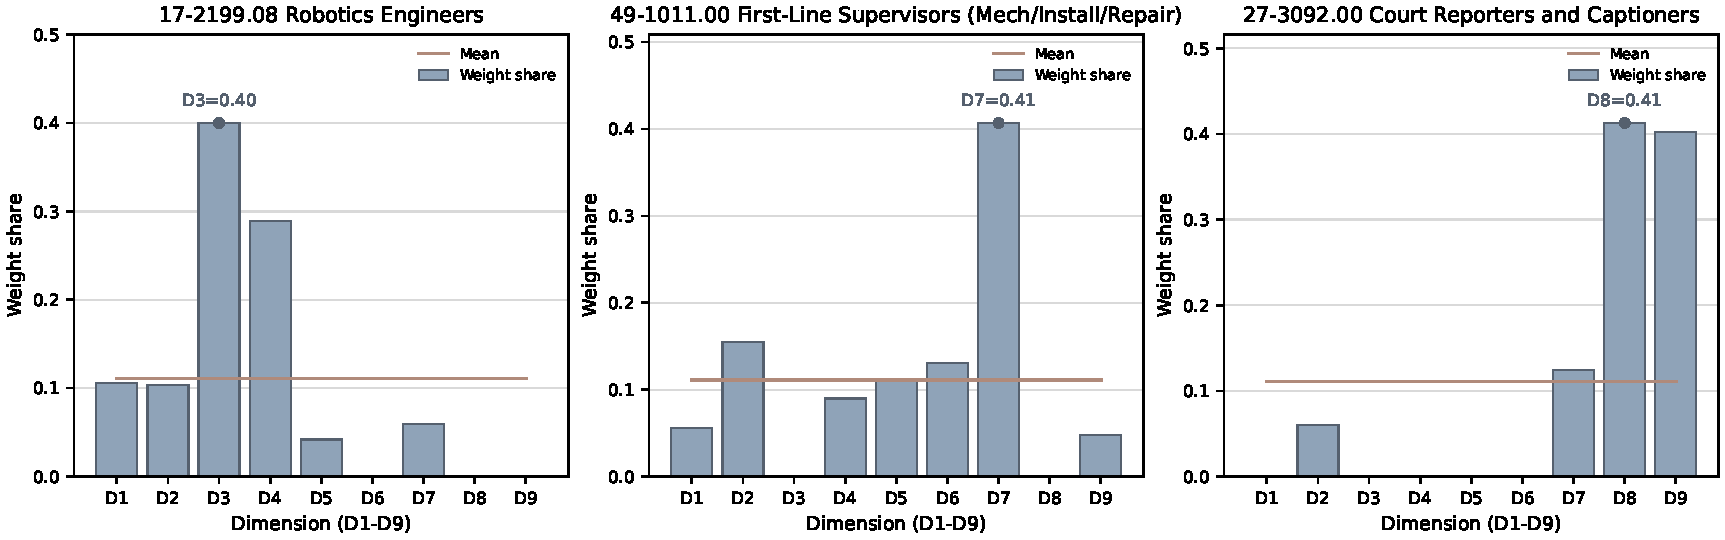
\includegraphics[width=0.98\textwidth]{figures/task_dna_genai_mapping_triptych.pdf}
% \caption{基于GenAI能力$\rightarrow$任务映射数据的职业DNA维度权重分布（D1--D9）。三幅子图分别对应职业 17-2199.08、49-1011.00 与 27-3092.00；柱高表示任务权重在能力维度上的占比，水平线表示维度均值，标注点为主导维度。}
% \label{fig:task_dna_genai_mapping_triptych}
% \end{figure}
% 在此简单分析上图：分析分析分析分析分析分析分析分析分析分析分析分析分析分析分析分析分析分析分析分析分析分析分析分析分析分析分析分析分析分析分析分析分析分析分析分析分析分析分析分析分析分析分析分析分析分析分析分析分析分析分析分析分析分析分析分析分析分析分析分析分析分析分析分析分析分析\\

基于上表得到的$s,c$数据，绘制\textbf{权威 $s,c$ 档位分布图}。该图的作用是\emph{揭示GenAI对该职业的潜在冲击模式}：若多数任务落在高 $s$ 低 $c$ 区域，表明该职业面临较高的自动化替代风险；反之，若多数任务落在低 $s$ 高 $c$ 区域，则GenAI更可能增强而非替代人类工作。

\begin{figure}[H]
\centering
\begin{minipage}{0.32\linewidth}
    \centering
    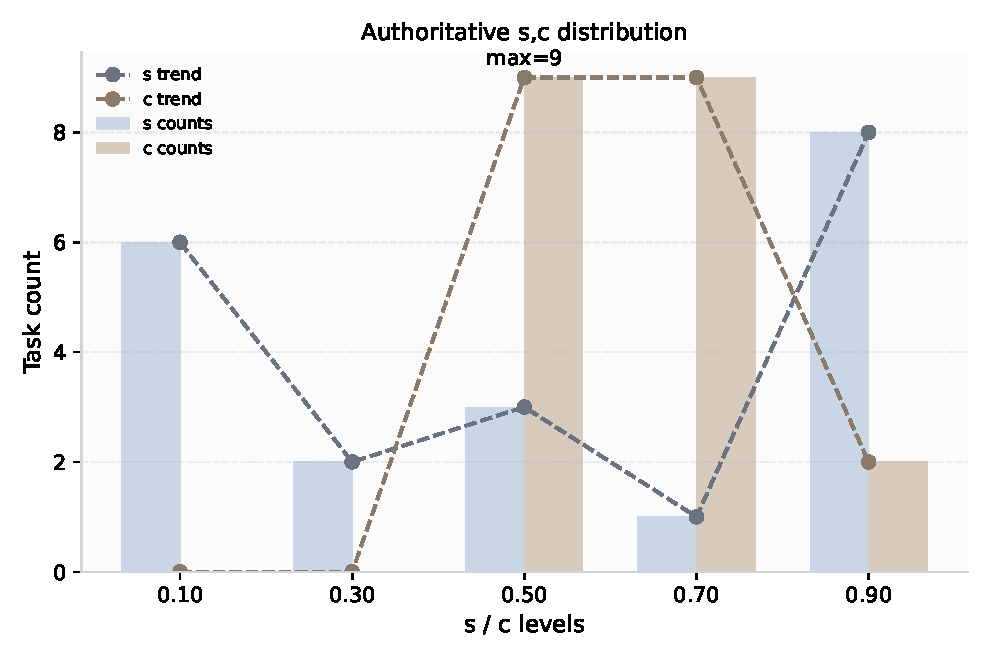
\includegraphics[width=\linewidth]{figures/task_dna_17-2199.08_authoritative_sc_distribution.pdf}\\
    \small (a) 17-2199.08 机器人工程师
\end{minipage}\hfill
\begin{minipage}{0.32\linewidth}
    \centering
    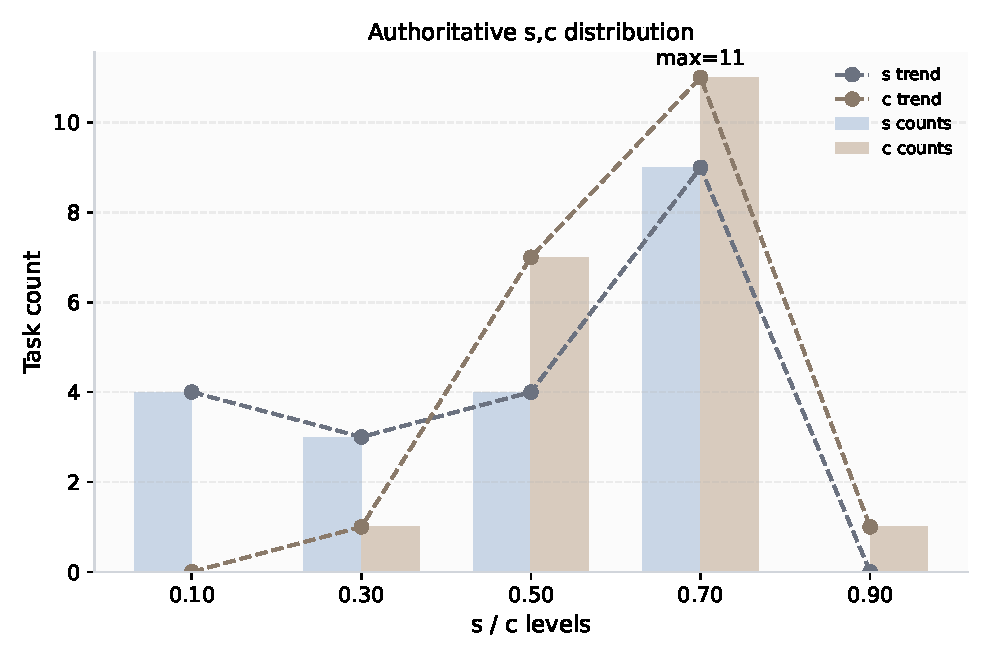
\includegraphics[width=\linewidth]{figures/task_dna_49-1011.00_authoritative_sc_distribution.pdf}\\
    \small (b) 49-1011.00 一线主管
\end{minipage}\hfill
\begin{minipage}{0.32\linewidth}
    \centering
    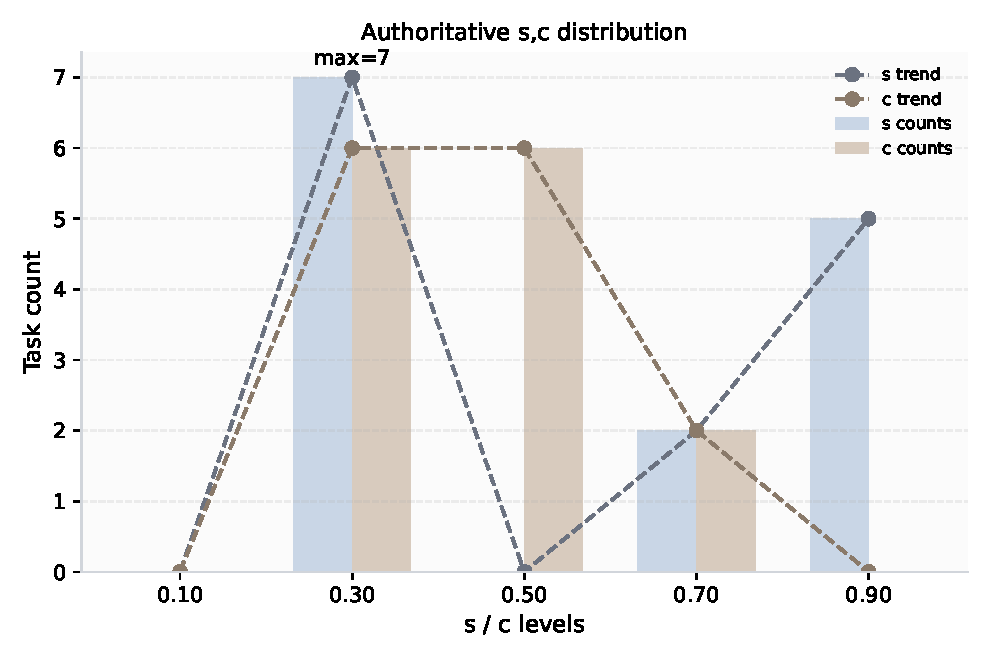
\includegraphics[width=\linewidth]{figures/task_dna_27-3092.00_authoritative_sc_distribution.pdf}\\
    \small (c) 27-3092.00 法庭速录
\end{minipage}
\caption{三职业的权威 $s,c$ 档位分布对比。（a）机器人工程师：$c$ 向高档位偏移，呈增强型冲击；（b）一线主管：$s,c$ 分布分散，冲击方向不单一；（c）法庭速录：$s$ 呈两端分化，高频核心任务接近替代型冲击。}
\label{fig:task_dna_sc_triptych}
\end{figure}

结合图~\ref{fig:task_dna_sc_triptych}，我们从 $(s_{ij},c_{ij})$ 的结构分布解释三类职业的冲击机制。目的是为了和预测之后的结果进行呼应。对\textbf{机器人工程师}，$c$ 的质量明显集中在中高档位，说明 GenAI 更偏向以增强的方式赋能工作流。

对\textbf{一线主管（机械/安装/维修）}，$s$ 与 $c$ 的分布更分散且无单一高峰，这与其任务 DNA 的多元性一致，意味着 GenAI 在不同子任务上呈“局部替代+局部增强”的混合效应，结构变化更依赖多任务的累积贡献。对\textbf{法庭速录与字幕}，$s$ 在高档位的集中度更高且与高频任务耦合更紧，显示其核心任务更接近可自动化文本处理范畴，模型上表现为负 $\mu^{task}_{ij}$ 任务权重占比更高，结构重排更快、更早触发任务份额下沉。

$\mu^{task}_{ij}>0$ 表示GenAI更可能增强该任务（提高产出/质量/速度），$\mu^{task}_{ij}<0$ 表示该任务更可能被替代或显著压缩。

得到$(s_{ij},c_{ij})$ 数据之后，变可以进一步汇总了三职业中负净冲击任务（$\mu^{task}_{ij}<0$）的权重与典型任务，结果见表~\ref{tab:task_sc_negative_impact} 
负净冲击（被替代倾向）

\begin{table}[H]
\centering
\caption{三职业负净冲击任务（$\mu^{task}_{ij}<0$）汇总}
\label{tab:task_sc_negative_impact}
\small
\begin{tabular}{llccc}
\toprule
\textbf{SOC} & \textbf{职业名称} & \textbf{负冲击任务数} & $\sum_{j:\mu_{ij}<0} w_{ij}$ & \textbf{典型任务（task\_id, $w$, $\mu$, dims）} \\
\midrule
17-2199.08 & 机器人工程师 & 8 & 0.400 & 16521/16516/21057/16528等，$\mu=-0.20$，D3 \\
49-1011.00 & 一线主管（机械维修） & 1 & 0.059 & 2912, 0.059, $-0.20$, D5 \\
27-3092.00 & 法庭速录与字幕 & 5 & 0.413 & 8653/21183/8663/8656/8657，$\mu=-0.40$，D8 \\
\bottomrule
\end{tabular}
\end{table}

\begin{itemize}
    \item \textbf{机器人工程师}：负净冲击权重总和为 0.400，8 项任务均落在 D3（算法编程与自动化），$\mu=-0.20$。这意味着该职业约 40\% 的核心任务存在可自动化压力，但净冲击幅度相对温和（$s=0.90,c=0.70$），体现为"高替代但仍有较强增强"的编码类任务。也就是说强强抵消了。
    \item \textbf{一线主管}：仅 1 项任务（调度排程，task\_id=2912）呈负净冲击，权重仅 0.059，落在 D5（规划与流程调度），$\mu=-0.20$。该职业的核心任务更多落在监督、培训与协调维度（D6/D7），与人类技能形成互补，整体替代风险最低。
    \item \textbf{法庭速录与字幕}：负净冲击权重总和高达 0.413，5 项任务集中落在 D8（语言理解与文本生成），$\mu=-0.40$，远高于其他两职业。这表明该职业的核心任务（速记、转写、校对）高度集中于语言自动化维度，GenAI 替代效应最强，预期将在后续动态演化中更早出现"任务份额跌破阈值"的时间点。
\end{itemize}

基于以上对职业核心组成任务（Top Task DNAN）、Gen-AI能力维度匹配以及正负冲击强度的分析，我们可以回答题目的问题：在Gen-AI时代，哪些驱动因素会造成职业的变化？
这部分交给你们。

\subparagraph{Robotics Engineers (O*NET 17-2199.08)}
GenAI 与机器人平台、仿真环境及基础模型的集成显著提升了工具链能力，从而加速采用（$A(t)\uparrow$）。在任务层面，文档撰写、常规代码生成及测试等任务更容易被替代（$s_{ij}$ 较高），而系统级设计与现场集成任务的替代速度相对较慢。公开报道显示，主流机器人平台已开始集成生成式 AI 以加速开发与部署~\cite{nvidia_isaac_2024}，为 driver 存在性提供了经验证据。

\subparagraph{First-Line Supervisors of Mechanics (O*NET 49-1011.00)}
预测性维护、智能诊断与排程优化工具的成熟推动了采用上升（$A(t)\uparrow$）。受此影响，"诊断信息汇总""调度沟通""例行检查"等任务结构被重排：部分文书与记录任务权重下降，而需要现场判断与人员协调的任务相对上升。权威企业研究解读将预测性维护与工业 AI 列为制造与运营领域的关键应用~\cite{mckinsey_maintenance_2023}，支撑了该职业的 driver 机制。

\subparagraph{Court Reporters and Simultaneous Captioners (O*NET 27-3092.00)}
自动语音识别（ASR）与转写/字幕自动化技术的进步提升了速度与一致性，推动采用上升（$A(t)\uparrow$）。任务结构因此分化："实时转写""初稿校对""格式化""归档"等任务更多由自动化系统承担，而人类从业者转向校验、法律语境判断与质量控制。行业趋势报告明确指出，自动化与 AI 正在显著提升法庭记录流程的速度与准确性~\cite{ncra_trends_2024}。

\subsubsection{将“发展轨迹”与“任务需求”紧密耦合：开始对未来的任务权重进行预测}

题目要求“given the current trajectory and expected impacts of Gen-AI”，其中“current trajectory”我们将其定义为外生的采纳路径 $A(t)\in[0,1]$ 表示在时间 $t$ ，Gen-AI的采用率。并且，0被视为当前时间点，意味着从当前到未来的跨度。

考虑到模型的适用性以及准确性，我们不对未来的任何时间点进行任何的定量预测，转而从更本质的角度出发，以任务\textbf{相对份额}作为预测对象，
定义未归一化任务权重

\begin{equation}
    q_{ij}(t)=w_{ij}\Big[(1-A(t))+A(t)\exp\big(\eta\,\mu^{task}_{ij}\big)\Big],
\end{equation}
其中 $\eta>0$ 为冲击强度缩放（无量纲），用于刻画“ai采用率带来的任务结构重排幅度”，并在敏感性分析中报告其影响。\\
直观上，在 $A(t)=0$ 时，只剩下 $w_{ij}$，任务权重与当前保持一致；在 $A(t)$ 增大时，由于右侧部分对任务权重施加了一个与 $\mu^{task}_{ij}$ 单调一致的乘性变换（保证权重为正），任务层净冲击 $\mu^{task}_{ij}$ 逐步释放，任务需求结构随之重排。


然后将 $q_{ij}(t)$ 归一化就可以得到任务的相对份额。
\begin{equation}
    p_{ij}(t)=\frac{q_{ij}(t)}{\sum_{k=1}^{J_i} q_{ik}(t)}.
\end{equation}

当 $A(t)$ 上升（GenAI采用率增大）时，若 $\mu^{task}_{ij}<0$，则 $q_{ij}(t)$ 相对缩小，$p_{ij}(t)$ 下降；反之若 $\mu^{task}_{ij}>0$，则该任务份额上升。

% \paragraph{未来时间点}
% 结合前述定义，任务的有效归零时间仍为
% \begin{equation}
%     \tau_{ij}(\epsilon)=\min\{t:\ p_{ij}(t)\le \epsilon\}.
% \end{equation}
% 通过对Top任务的 $\tau_{ij}(\epsilon)$ 进行比较，我们可以直接回答：在不同采纳情景下，哪些任务会最先"消失"，哪些任务会长期保留，从而给出对该职业"未来"形态变化的可解释预测。

那么对于任意两个时间点 $t_0,t_1$，任务 $j$ 的份额变化定义为
\begin{equation}
\label{eq:delta_p}
r_{ij}(t_0,t_1)=\left|\Delta p_{ij}(t_0,t_1)\right|=p_{ij}(t_1)-p_{ij}(t_0).
\end{equation}

按 $r_{ij}$ 降序排列，可识别出对结构变化贡献最大的任务（Top contributors）。该指标取代原先"按均值选取 TopK"的方式，避免挑到稳定大头而掩盖结构重排。

\paragraph{(ii) Top-$m$ 换血率}

定义职业的核心任务集为按 $p_{ij}(t)$ 降序的前 $m$ 个任务，记为 $\mathrm{Top}_m(p_i(t))$。换血率衡量核心任务集合的更替程度：
\begin{equation}
\label{eq:turnover}
J_i(t_0,t_1;m)=1-\frac{\left|\mathrm{Top}_m(p_i(t_0))\cap \mathrm{Top}_m(p_i(t_1))\right|}{m}.
\end{equation}
当 $J_i=0$ 时，核心任务集完全不变；当 $J_i=1$ 时，核心任务集完全换血。

\paragraph{(iv) 排名翻转与归一化翻转强度}
令 $\mathrm{rank}_i(j,t)$ 表示任务 $j$ 在职业 $i$ 中按 $p_{ij}(t)$ 降序的名次（1 为最高）。定义翻转对数为
\begin{equation}
\label{eq:inversion_count}
I_i(t_0,t_1)=\#\{(a,b):\ \mathrm{rank}_i(a,t_0)<\mathrm{rank}_i(b,t_0)\ \wedge\ \mathrm{rank}_i(a,t_1)>\mathrm{rank}_i(b,t_1)\}.
\end{equation}
该指标计数"在 $t_0$ 时 $a$ 排在 $b$ 前面，但在 $t_1$ 时 $a$ 落到 $b$ 后面"的任务对数目。为便于跨职业比较，我们进行归一化：
\begin{equation}
\label{eq:normalized_inversion}
\widetilde I_i(t_0,t_1)=\frac{2I_i(t_0,t_1)}{N_i(N_i-1)}\in[0,1],
\end{equation}
其中 $N_i$ 为职业 $i$ 的任务总数。$\widetilde I_i$ 的工作职责是：作为Kendall $\tau$ 距离的归一化形式，刻画任务相对重要性序列的结构性扰动程度。

\paragraph{职业重新定义的综合判据}
我们采用结构指标作为"职业已重新定义"的主要判据：
\begin{equation}
\label{eq:redefinition_trigger}
\text{结构已重定义} \Longleftrightarrow \widetilde I_i(t_0,t_1) \ge \theta_{I} \quad \text{或} \quad J_i(t_0,t_1;m) \ge \theta_{J},
\end{equation}
其中 $\theta_{I}\in(0,1)$ 为翻转强度阈值（例如 $\theta_{I}=0.15$），$\theta_{J}\in(0,1)$ 为换血率阈值（例如 $\theta_{J}=0.40$），$m$ 为核心任务数（例如 $m=5$）。

阈值 $\theta_{I}$、$\theta_{J}$ 不作为固定常数，我们在多个阈值设置下计算结果，展示结论的稳健性区间。\\
这部分也要做敏感性分析，给出鲁棒区间。\\这部分也要做敏感性分析，给出鲁棒区间。

\paragraph{结构指标的可视化}
我们据此构建两类核心可视化：
\begin{enumerate}
  \item \textbf{排名翻转图}（图~\ref{fig:rank_flip_stem}）：连线两端分别为 $\mathrm{rank}_i(j,t_0)$ 与 $\mathrm{rank}_i(j,t_1)$，翻转幅度越大、线越陡，结构性重排越显著。
  \item \textbf{贡献分解瀑布图}（图~\ref{fig:rank_flip_stem} 右）：按 $r_{ij}$ 降序展示 Top contributors 对总份额变化的累积贡献。
\end{enumerate}

\begin{figure}[H]
\centering
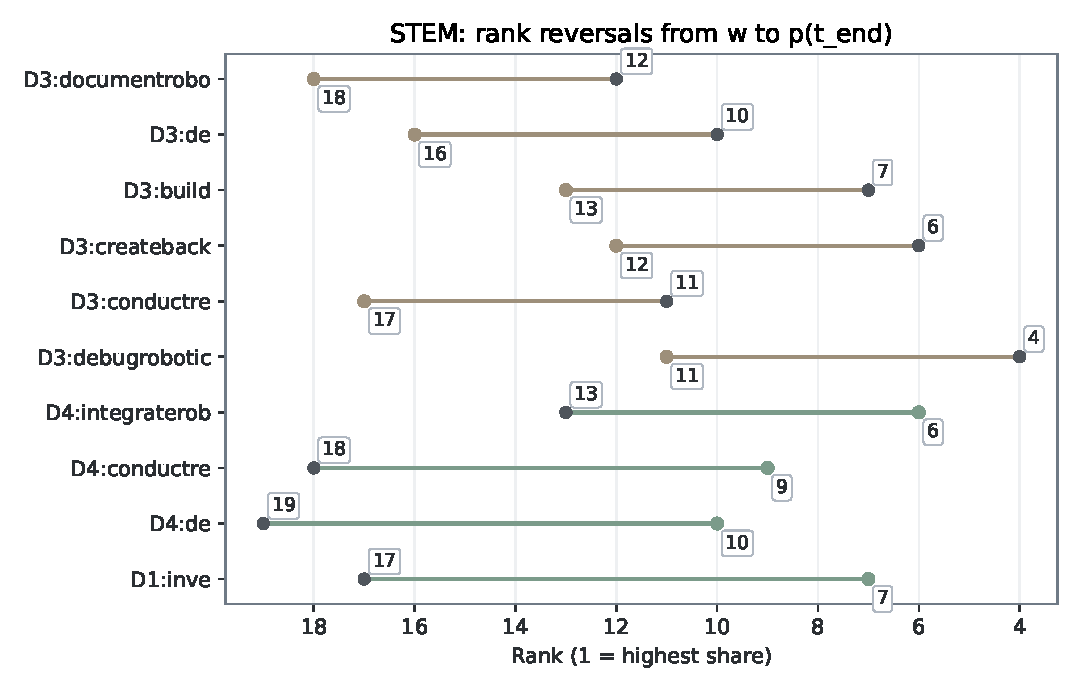
\includegraphics[width=0.95\linewidth]{figures/fig_STEM_rankflip_contribution_v2.pdf}
\caption{STEM职业（17-2199.08）从基线（$t_0=0$, $A=0$）到末期（$t_1=2040$）的排名翻转。连线两端分别为 $\mathrm{rank}_i(j,t_0)$ 与 $\mathrm{rank}_i(j,t_1)$，翻转幅度越大、线越陡，结构性重排越显著。STEM职业（17-2199.08）结构变化的 Top contributors 贡献分解。按 $r_{ij}$ 降序展示各任务对总份额变化的累积贡献，揭示结构重排的主要驱动任务。}
\label{fig:rank_flip_stem}
\end{figure}

\subsection{教育项目推荐与Gen-AI整合策略}
\label{subsec:task3_programs}

基于前述职业选择及其任务层面的Gen-AI影响分析，我们为三个代表性职业推荐具体的教育项目。
推荐遵循三重准则：\textbf{（1）机构层面的行业领导力}、\textbf{（2）课程与产业需求的对齐度}、以及\textbf{（3）Gen-AI资源整合的制度化路径}。
具体推荐项目及其详细选择依据见附录表~\ref{tab:programs_genai_rationale}。

针对\textbf{机器人工程师}，我们推荐卡内基梅隆大学机器人研究院的MRSD项目，该项目具备行业领导力且已建立Gen-AI课程资源接口。
针对\textbf{机械维修一线主管}，Universal Technical Institute（UTI）展现出快速响应产业技术迁移的能力，并已将AI诊断纳入教学叙事。
针对\textbf{法庭速录师}，Generations College作为美国首创法庭速录项目的历史传承者，其Realtime训练体系可与Gen-AI后编辑工具形成互补。

\subsubsection{基于文本的课程剪枝与增补元模型}

在完成项目选择后，我们进一步构建一个\textbf{纯文本驱动的课程优化元模型}，用于指导各教育项目如何在Gen-AI时代进行课程结构调整。该模型仅依赖课程标题与描述文本，无需学分信息，具备高度可解释性与可迁移性。

\paragraph{三轴评估框架}
我们为每门课程 $m$ 构造三个可解释的代理指标：

\textbf{（1）就业轴 $E_m$}：衡量课程文本与劳动力市场技能需求的对齐程度。该指标通过统计课程描述中命中预定义就业关键词词典 $\mathcal{K}_E$ 的频次并归一化获得：
\\这部分是必要的，不能过于理想主义，仍然需要结合真实的社会形态。
\begin{equation}
E_m = \text{norm}\left(\sum_{w \in \mathcal{K}_E} \mathbf{1}[w \in t_m]\right)
\end{equation}
其中 $t_m$ 为课程 $m$ 的文本内容（标题 + 描述）。该指标的作用类似于\textbf{职业相关性过滤器}，识别与产业技能直接挂钩的课程模块。

\textbf{（2）人文轴 $H_m$}：衡量课程对批判性思维、伦理意识、跨学科素养等人文能力的贡献程度：
\begin{equation}
H_m = \text{norm}\left(\sum_{w \in \mathcal{K}_H} \mathbf{1}[w \in t_m]\right)
\end{equation}
人文轴的引入是对"唯就业论"的关键修正——我们认为，Gen-AI时代恰恰需要强化人类独有的判断力与价值观锚定能力。

\textbf{（3）冗余度 $R_m$}：捕捉课程与同一项目中其他课程的内容重叠程度：
\begin{equation}
R_m = \max_{n \neq m} \text{sim}(t_m, t_n)
\end{equation}
该指标识别"信息熵最低"的模块——即那些可被其他课程替代的冗余内容。

\paragraph{剪枝决策规则}
我们采用\textbf{三重门槛联合约束}的保守剪枝策略：仅当一门课程同时满足"就业相关性低"、"人文贡献低"、"与其他课程高度冗余"三个条件时，才建议将其从课程体系中移除：
\begin{equation}
\text{PRUNE}(m) = \mathbf{1}\left[(E_m < e_{\min}) \land (H_m < h_{\min}) \land (R_m > r_{\min})\right]
\end{equation}
课程保留决策变量定义为 $x_m = 1 - \text{PRUNE}(m)$。这种设计确保了我们不会误删那些"就业导向弱但人文价值高"的课程——例如伦理学、科技史等在AI时代反而更加重要的模块。

\paragraph{增补建议机制}
在剪枝的同时，模型检测整体人文轴均值是否低于目标区间：
\begin{equation}
\overline{H} = \frac{1}{M} \sum_{m} H_m
\end{equation}
若 $\overline{H}$ 低于阈值，模型建议新增特定类型的模块集合 $\Delta\mathcal{M}$，以提升课程体系的人文素养覆盖度。增补建议的具体内容依据各职业的Gen-AI影响特征动态生成。

\paragraph{模型局限与缓解措施}
当课程描述过短或偏向营销性语言时，$E_m$ 与 $H_m$ 可能被低估。我们通过以下方式缓解该问题：（1）允许手动扩充关键词词典；（2）报告阈值参数的敏感性区间，供决策者参考调整。


